
% ════════════════════════════════════════════
% 单个问题的建立求解（5.X.问题X.tex，二级标题包装）—— 写作提示词见本文件末尾【本章节写作提示词】。
% ════════════════════════════════════════════
\subsection{问题一的模型的建立和求解}


% ════════════════════════════════════════════
% 具体分析（5.1.1.具体分析.tex，三级子块）
% ════════════════════════════════════════════
\subsubsection{具体分析}

针对问题一，本问属于确定性线性优化类问题，采用线性规划方法对微网一天的购电与储能充放电策略进行联合优化求解。

本文先对附件一提供的单日分时电价、小区负载与光伏预测数据进行读取与时间对齐，将其整理为一天 144 个 10 分钟时间间隔上的功率序列；依据储能设备的容量、充放电功率与效率约束，将一天内的能量平衡关系与储能荷电状态递推关系写成线性约束；以全天购电费用最小为目标函数，加入储能设备在 0:00 与 24:00 储电量相等的日循环约束，并按附录1给定值固定 0:00 储电量为 6000 kWh，构建标准线性规划模型；最后调用线性规划求解器求得每个时间间隔的购电功率与储能充放电功率，进而得到全天购电量、购电费以及各时段储能充放电量。具体分析流程如图\ref{fig:analysis1_flow}所示。

\begin{figure}[H]
    \begin{center}
        \begin{tikzpicture}[x=1cm, y=0.75cm,
            flowhead/.style={rectangle, rounded corners=3pt, draw=blue!70!black, fill=blue!55!black, text=white, font=\bfseries, minimum width=7.2cm, minimum height=1.1cm, align=center, inner sep=2pt, line width=0.7pt},
            flowbox/.style={rectangle, rounded corners=2.5pt, draw=blue!65!black, fill=blue!12, minimum width=7.2cm, minimum height=1.0cm, align=center, inner sep=2pt, line width=0.6pt},
            flowend/.style={rectangle, rounded corners=2.5pt, draw=blue!75!black, fill=blue!45!black, text=white, font=\bfseries, minimum width=7.2cm, minimum height=1.0cm, align=center, inner sep=2pt, line width=0.7pt},
            flowarrow/.style={thick, -{Stealth}, blue!60!black}
        ]
            \node[flowhead] at (0, 0) (h) {问题一：单日线性规划建模与求解};
            \node[flowbox] at (0, -1.8) (s1) {\textbf{读取单日数据}\\\footnotesize 负荷 · 光伏 · 分时电价};
            \node[flowbox] at (0, -3.6) (s2) {\textbf{时间对齐}\\\footnotesize 整理为 144 个 10 分钟间隔};
            \node[flowbox] at (0, -5.4) (s3) {\textbf{设定决策变量}\\\footnotesize 购电功率与储能充放电功率};
            \node[flowbox] at (0, -7.2) (s4) {\textbf{整理运行约束}\\\footnotesize 储能容量 / 充放电功率 / 效率};
            \node[flowbox] at (0, -9.0) (s5) {\textbf{建立目标函数}\\\footnotesize 全天购电费用最小};
            \node[flowbox] at (0, -10.8) (s6) {\textbf{固定储电初值并施加日循环}\\\footnotesize $E_0=6000$ kWh · SOC 在 0:00 与 24:00 相等};
            \node[flowbox] at (0, -12.6) (s7) {\textbf{构建并求解线性规划}\\\footnotesize 调用线性规划求解器};
            \node[flowend] at (0, -14.4) (s8) {输出最优策略\\\footnotesize 购电量 · 购电费 · 充放电量};
            \draw[flowarrow] (h) -- (s1);
            \draw[flowarrow] (s1) -- (s2);
            \draw[flowarrow] (s2) -- (s3);
            \draw[flowarrow] (s3) -- (s4);
            \draw[flowarrow] (s4) -- (s5);
            \draw[flowarrow] (s5) -- (s6);
            \draw[flowarrow] (s6) -- (s7);
            \draw[flowarrow] (s7) -- (s8);
        \end{tikzpicture}
        \caption{问题一分析流程图}
        \label{fig:analysis1_flow}
    \end{center}
\end{figure}


% ════════════════════════════════════════════
% 模型准备（5.1.2.模型准备.tex，三级子块）
% ════════════════════════════════════════════
\subsubsection{模型准备}

\textbf{1.数据预处理}

附件一给出了某一天不同时刻的电价、小区负载和光伏发电预测功率，时间分辨率均为 10 分钟，其中末行时间记作 $0{:}00{+}1$，表示当天 24:00。原始数据以时间字符串索引，无法直接用于逐时段递推计算，因此需要先进行时间对齐与数值化处理。为便于后续建模，首先对数据进行预处理，具体步骤如下。

将一天划分为 144 个等长时间间隔，第 $k$ 个间隔对应时段 $[k\Delta t,(k+1)\Delta t]$，其中 $\Delta t=1/6$ 小时。设第 $k$ 个间隔的负载功率为 $L_k$、光伏功率为 $S_k$、电价为 $p_k$，则数据点 $(k+1)\Delta t$ 处记录的功率值即为该间隔内的平均功率，其能量可表示为：
\begin{equation}
    E_k = P_k\,\Delta t,\quad k=0,1,\dots,143
\end{equation}
其中，$E_k$ 表示第 $k$ 个间隔的能量（kWh），$P_k$ 为该间隔的功率（kW）。将时间边界 $0{:}00{+}1$ 映射为 24:00，并对三列数据统一执行数值化与缺失检查，预处理前后对比如图\ref{fig:preprocess1}所示。

\begin{figure}[H]
    \centering
    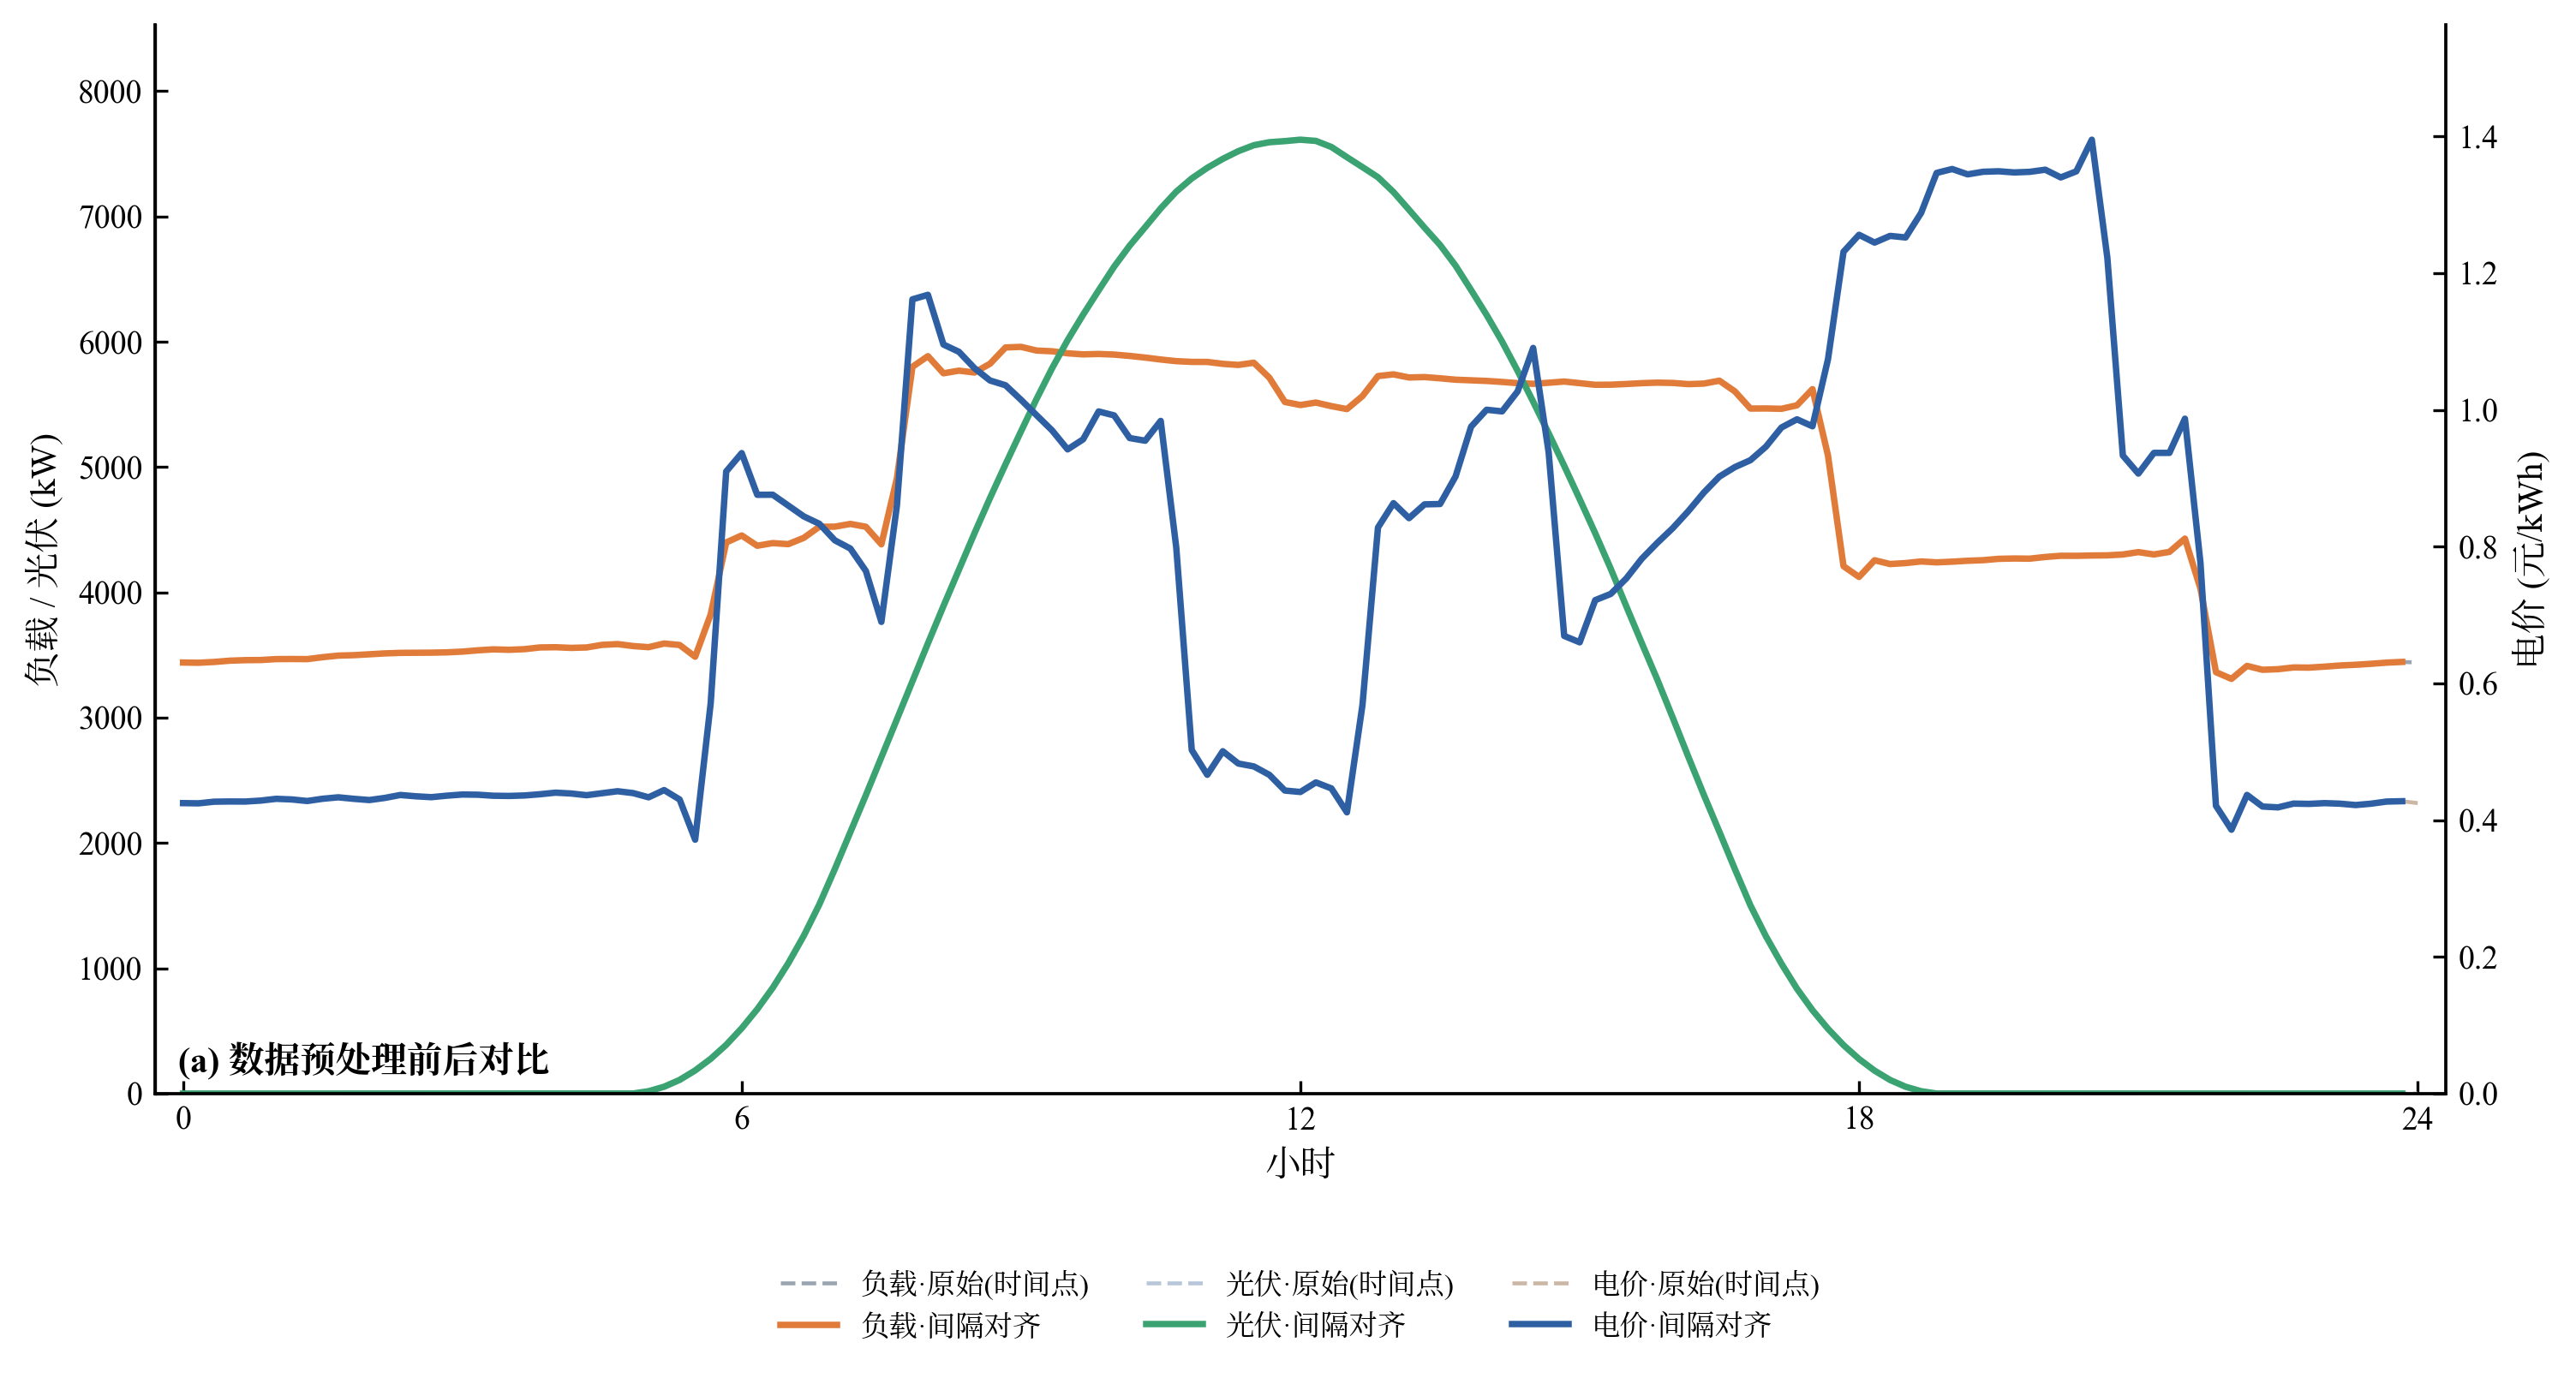
\includegraphics[width=0.72\textwidth]{../求解/问题一/图片/图1-1_预处理前后对比.png}
    \caption{问题一数据预处理前后对比}
    \label{fig:preprocess1}
\end{figure}

由图\ref{fig:preprocess1}可知，预处理后电价、负载与光伏三条曲线均被完整对齐到 144 个 10 分钟间隔上，数据无缺失、无异常，且光伏功率在日出后至日落前呈现典型的单峰形态，为后续优化提供了可靠的输入。

\textbf{2.算法选择}

在完成数据预处理后，本问需要在一组候选算法中确定购电与储能调度的求解方法。微网购电调度本质上是一个带线性约束的凸优化问题，可从求解精度、计算效率与全局最优性等维度比较枚举搜索、贪心算法和线性规划三种候选方法，如表\ref{tab:algo1}所示。

\begin{longtable}{>{\centering\arraybackslash}p{0.18\textwidth}>{\centering\arraybackslash}p{0.26\textwidth}>{\centering\arraybackslash}p{0.24\textwidth}>{\centering\arraybackslash}p{0.20\textwidth}}
  \caption{问题一算法对比}
  \label{tab:algo1} \\
  \toprule
  算法 & 全局最优性 & 计算效率 & 约束处理 \\
  \midrule
  \endfirsthead
  \caption{问题一算法对比（续）} \\
  \toprule
  算法 & 全局最优性 & 计算效率 & 约束处理 \\
  \midrule
  \endhead
  \bottomrule
  \endfoot
  枚举搜索 & 可保证 & 极低 & 一般 \\
  贪心算法 & 无保证 & 高 & 困难 \\
  线性规划 & 严格保证 & 高 & 直接建模 \\
\end{longtable}

如\ref{tab:algo1}所示，枚举搜索虽然理论上能找到最优解，但决策变量规模达数百个，计算量爆炸；贪心算法难以同时协调储能容量约束与日循环约束；而线性规划能够把所有线性约束与目标函数直接纳入模型，由单纯形法或内点法求得全局最优解\cite{si2009}，且求解速度极快。综合以上分析，本问选择线性规划算法进行求解。


% ════════════════════════════════════════════
% 模型建立（5.1.3.模型建立.tex，三级子块）
% ════════════════════════════════════════════
\subsubsection{模型建立}

针对问题一，本节将从能量平衡与储能状态递推的角度建立微网日购电计划的线性规划模型。具体过程如下。

\textbf{步骤1：决策变量与目标函数}

定义模型的决策变量。设第 $k$ 个间隔的购电功率为 $g_k$，储能充电功率为 $c_k$，放电功率为 $d_k$，储电量为 $E_k$，其中 $k=0,1,\dots,143$，$E_k$ 为第 $k$ 个间隔起始时刻的储电量。微网全天购电费用为目标函数，即各间隔购电能量与电价乘积之和：
\begin{equation}
    \min \; Z=\sum_{k=0}^{143} g_k\,p_k\,\Delta t
\end{equation}
其中，$g_k\geq 0$ 为购电功率，$p_k$ 为第 $k$ 个间隔的交易电价，$\Delta t$ 为时间步长。该目标函数线性地刻画了微网的经济诉求。

\textbf{步骤2：功率平衡约束}

微网在每个间隔内须满足小区负载的用电需求。由功率守恒，购电功率、光伏功率与储能放电功率之和须不低于负载功率与储能充电功率之和，即允许在光伏过剩时弃光：
\begin{equation}
    g_k + S_k + d_k - c_k \geq L_k,\quad k=0,1,\dots,143
\end{equation}
其中，$S_k$ 为光伏预测功率，$L_k$ 为小区负载功率，$c_k,d_k$ 分别为充、放电功率。由于光伏发电边际成本为零，最优解会自动优先消纳光伏，只有在光伏与储能放电不足时才从外网购电。

\textbf{步骤3：储能状态递推约束}

储能设备的荷电状态随充放电行为逐间隔更新。考虑到充、放电效率均为 $\eta$，充电时从外部吸收的能量只有 $\eta$ 倍存入电池，放电时向负荷释放单位能量需从电池取出 $1/\eta$ 倍能量，因此递推关系为：
\begin{equation}
    E_{k+1}=E_k+\eta\,c_k\,\Delta t-\frac{1}{\eta}\,d_k\,\Delta t,\quad k=0,1,\dots,143
\end{equation}
其中，$\eta=0.9$ 为储能充放电效率。储能设备须满足容量上下限约束：
\begin{equation}
    E_{\min}\leq E_k\leq E_{\max},\quad E_{\min}=1200,\; E_{\max}=10800
\end{equation}
同时充放电功率受储能变换器额定功率限制：
\begin{equation}
    0\leq c_k\leq P_{\max},\quad 0\leq d_k\leq P_{\max},\quad P_{\max}=5000
\end{equation}

\textbf{步骤4：储电初值与日循环约束}

附录1给定 2025 年 1 月 1 日 0:00 的储电量为 6000 kWh，故储能 0:00 储电量应固定为：
\begin{equation}
    E_0=6000
\end{equation}
同时，问题一要求储能设备在 0:00 与 24:00 的储电量相同，以保证相邻日策略的可重复性，故加入日循环约束：
\begin{equation}
    E_0=E_{144}
\end{equation}
综上所述，问题一的完整线性规划模型为：
\begin{equation}
    \min \; Z=\sum_{k=0}^{143} g_k\,p_k\,\Delta t
\end{equation}
\begin{equation}
    \mathrm{s.t.}\quad g_k+S_k+d_k-c_k\geq L_k
\end{equation}
\begin{equation}
    E_{k+1}=E_k+\eta\,c_k\,\Delta t-\frac{1}{\eta}\,d_k\,\Delta t
\end{equation}
\begin{equation}
    E_{\min}\leq E_k\leq E_{\max},\quad 0\leq c_k,d_k\leq P_{\max},\quad g_k\geq 0
\end{equation}
\begin{equation}
    E_0=6000,\quad E_0=E_{144}
\end{equation}
该模型共有 $4\times 144+1=577$ 个连续变量，其中 $E_0$ 由附录1固定为 6000 kWh；全部约束均为线性等式或不等式，属于标准的线性规划问题\cite{dantzig1963}，可用单纯形法或内点法精确求解，且所得解即全局最优解。

综上所述，本节完成了问题一优化模型的建立，得到了以全天购电费用最小为目标、以功率平衡与储能状态为约束的线性规划模型，接下来将基于此进行求解。


% ════════════════════════════════════════════
% 模型求解（5.1.4.模型求解.tex，三级子块）
% ════════════════════════════════════════════
\subsubsection{模型求解}

基于上述模型，本节利用附件一数据在 Python 环境下调用线性规划求解器进行求解。核心参数为 $\Delta t=1/6$ h、$\eta=0.9$、$E_{\min}=1200$ kWh、$E_{\max}=10800$ kWh、$P_{\max}=5000$ kW，并按附录1给定 $E_0=6000$ kWh。求解得到微网在指定时间段的购电量及全天购电量和购电费如表\ref{tab:结果1-1}所示，储能设备在指定时段的充放电量及储电量如表\ref{tab:结果1-2}所示。

分时电价与最优购电功率的对应关系如图\ref{fig:结果1-2}所示。可以看到，购电功率主要集中在夜间低电价时段，用于在低价区间补充负荷缺口并为储能充电；在电价高峰时段购电功率明显下降，说明储能放电有效替代了高价购电。

负荷、光伏、净负荷与储能充放电功率的时序关系如图\ref{fig:结果1-3}所示。可以看出，光伏功率在白天形成明显高峰，使净负荷在午间大幅下降甚至转负，此时储能吸收光伏盈余进行充电；而在夜间与傍晚负荷高峰，储能放电填补净负荷缺口，购电功率相应减小。

\begin{figure}[H]
    \centering
    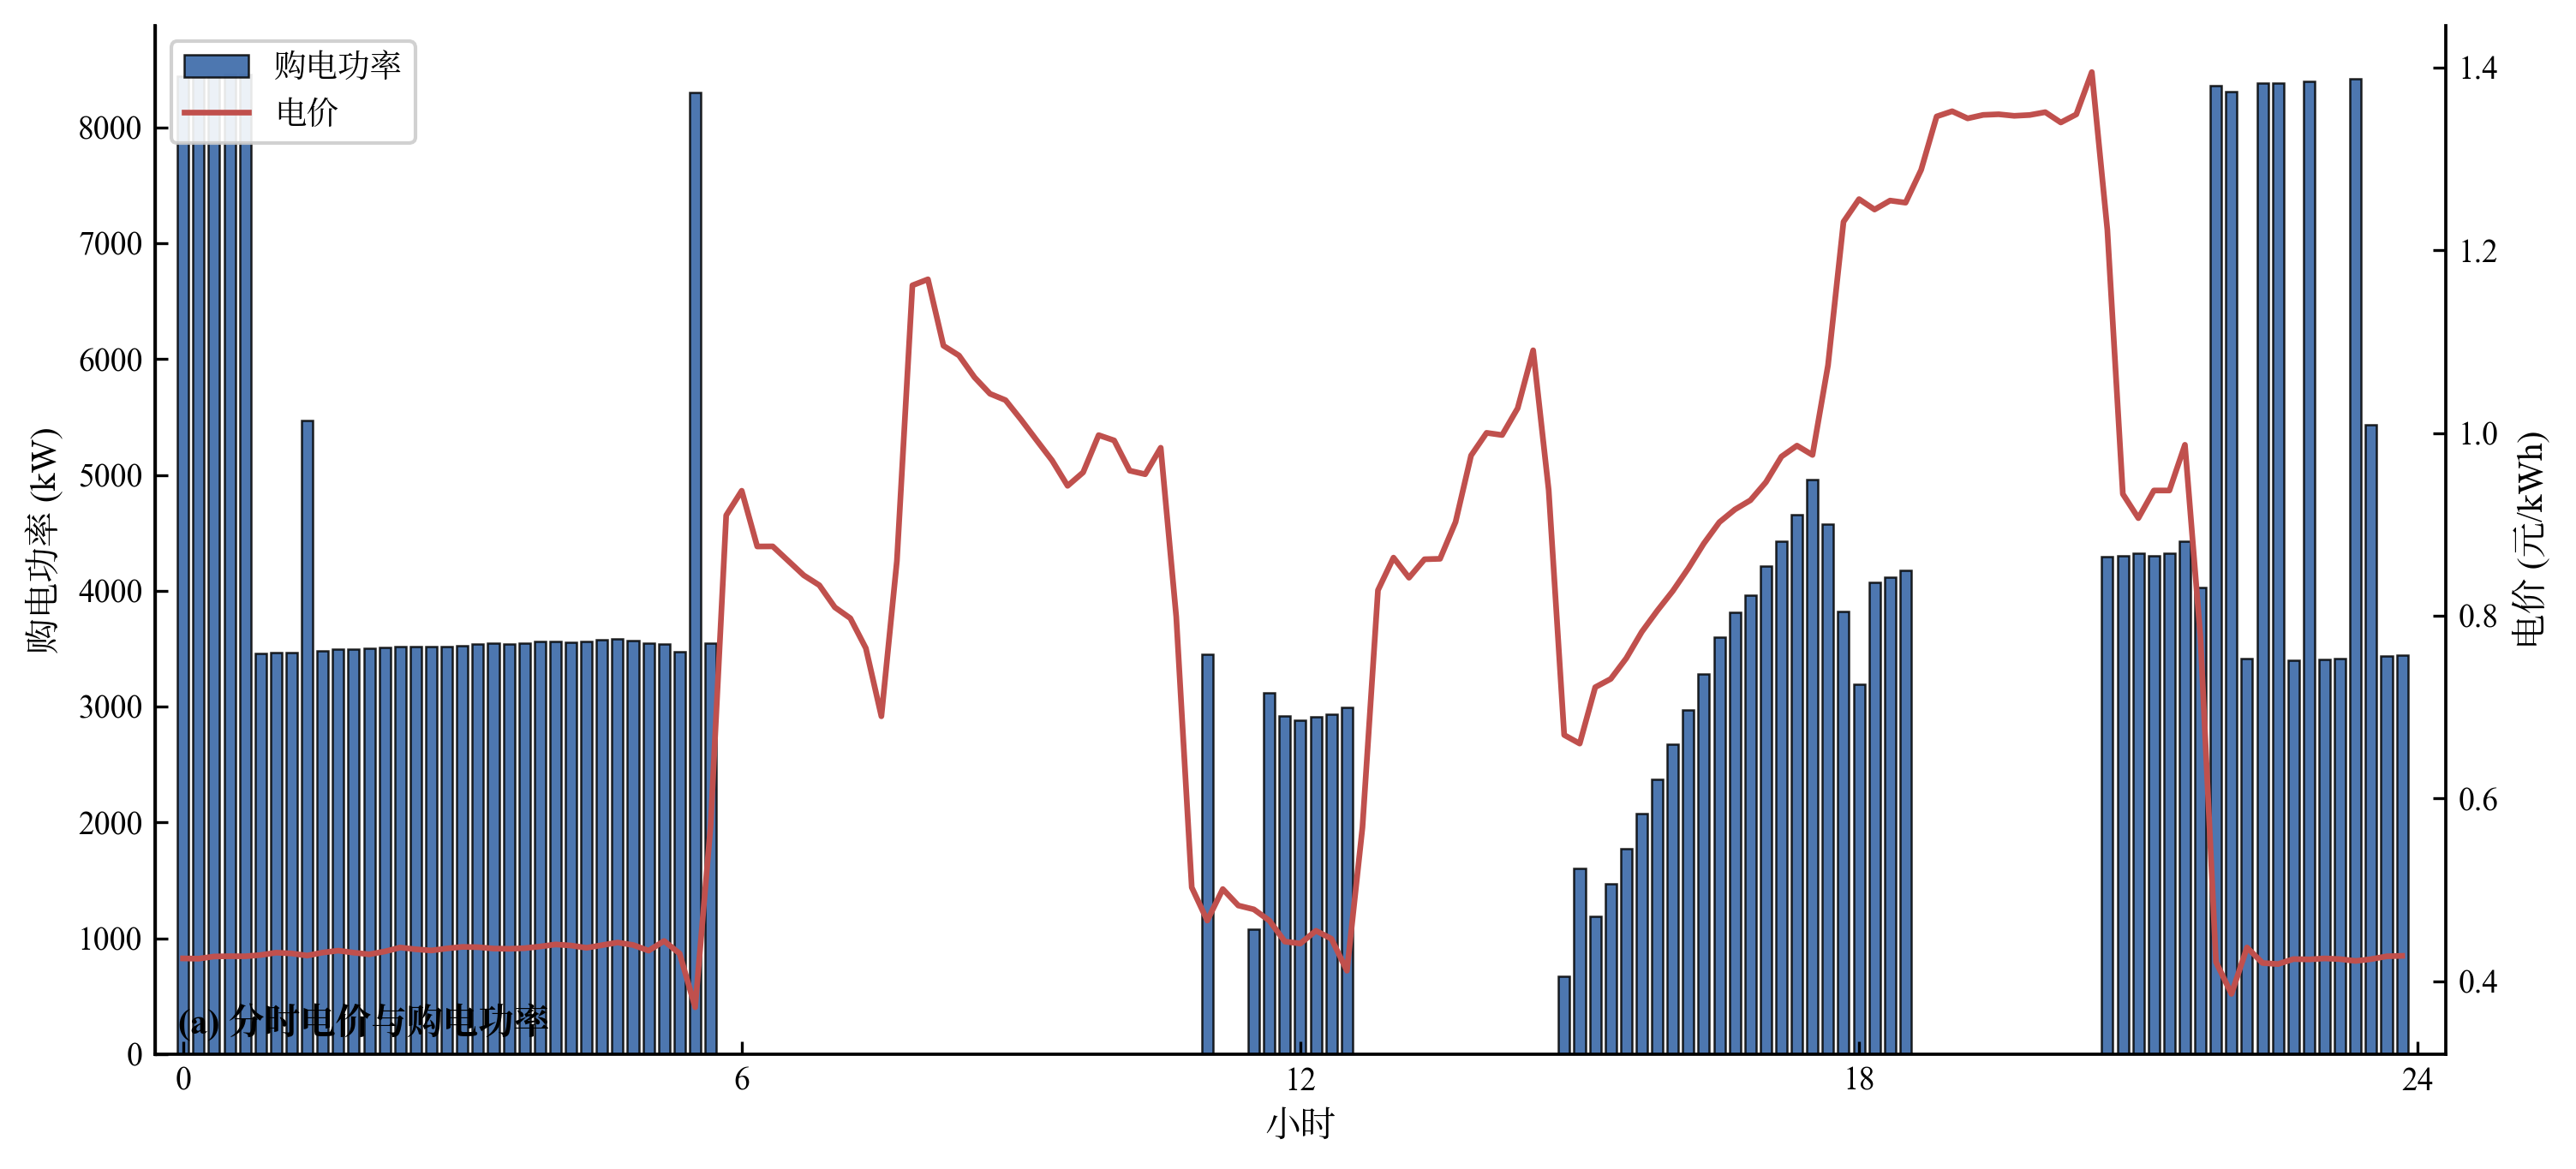
\includegraphics[width=0.65\textwidth]{../求解/问题一/图片/图1-2_电价与购电策略.png}
    \caption{分时电价与最优购电功率}
    \label{fig:结果1-2}
\end{figure}

\begin{figure}[H]
    \centering
    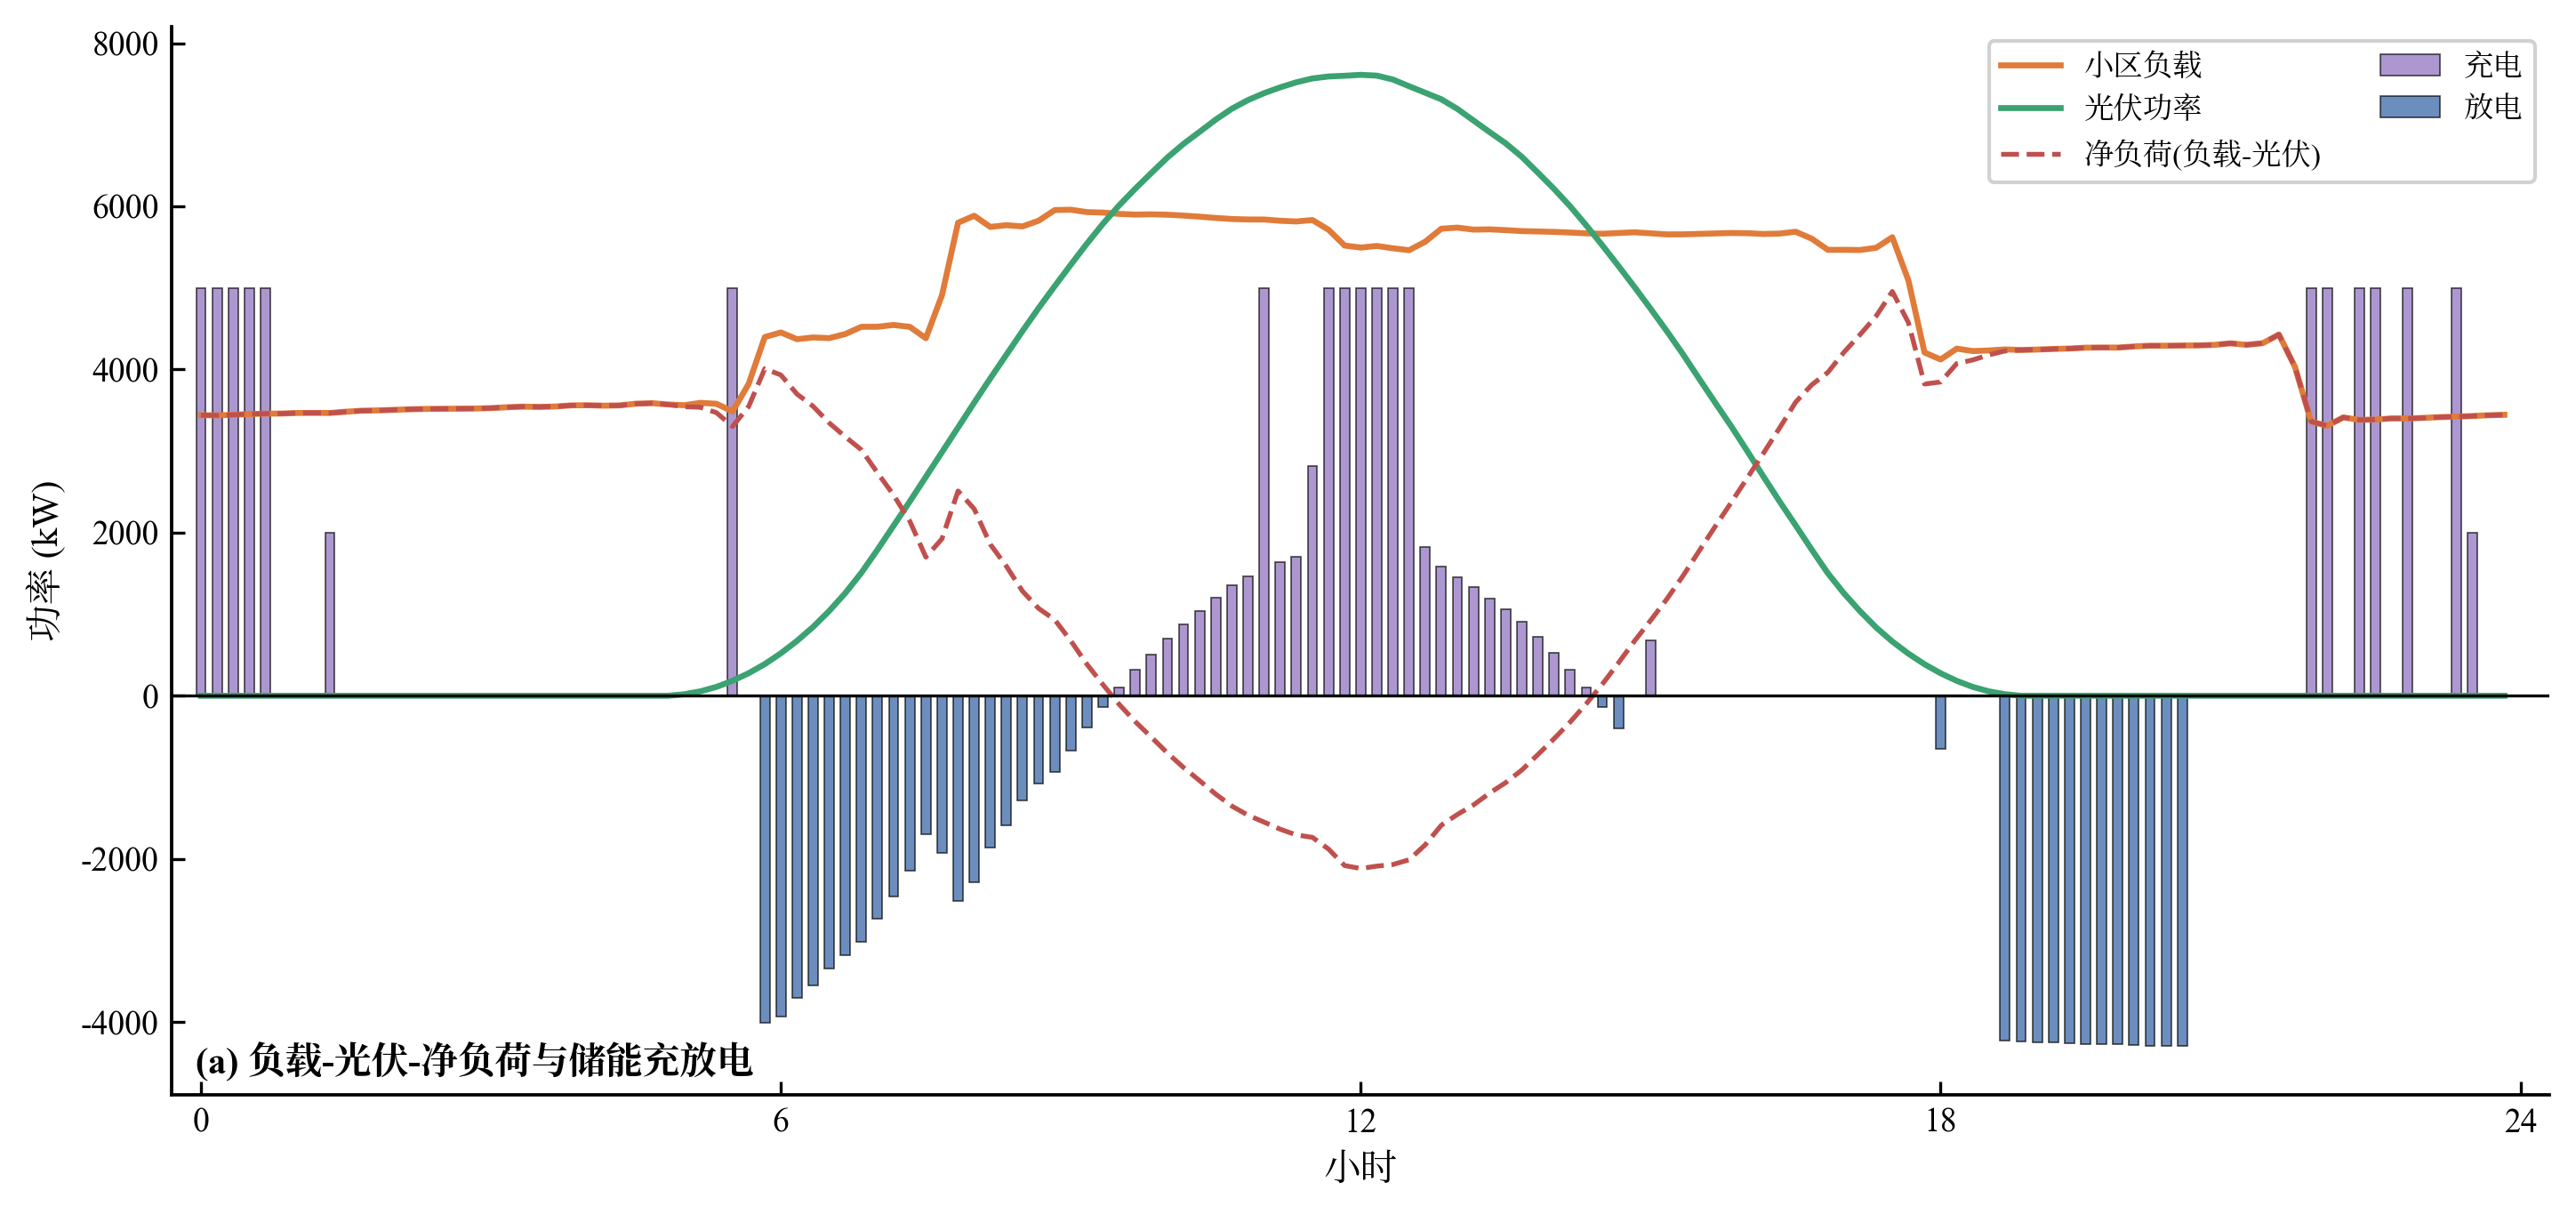
\includegraphics[width=0.65\textwidth]{../求解/问题一/图片/图1-3_负荷光伏净负荷与充放电.png}
    \caption{负荷、光伏、净负荷与储能充放电功率}
    \label{fig:结果1-3}
\end{figure}

储能设备的荷电状态轨迹与充放电功率如图\ref{fig:结果1-4}所示。储能荷电状态全程维持在 $[1200,10800]$ kWh 约束区间内，且在 0:00 与 24:00 处均精确等于附录1给定的 6000 kWh；充放电功率始终不超过 5000 kW 的额定限值，验证了模型的可行性。

\begin{figure}[H]
    \centering
    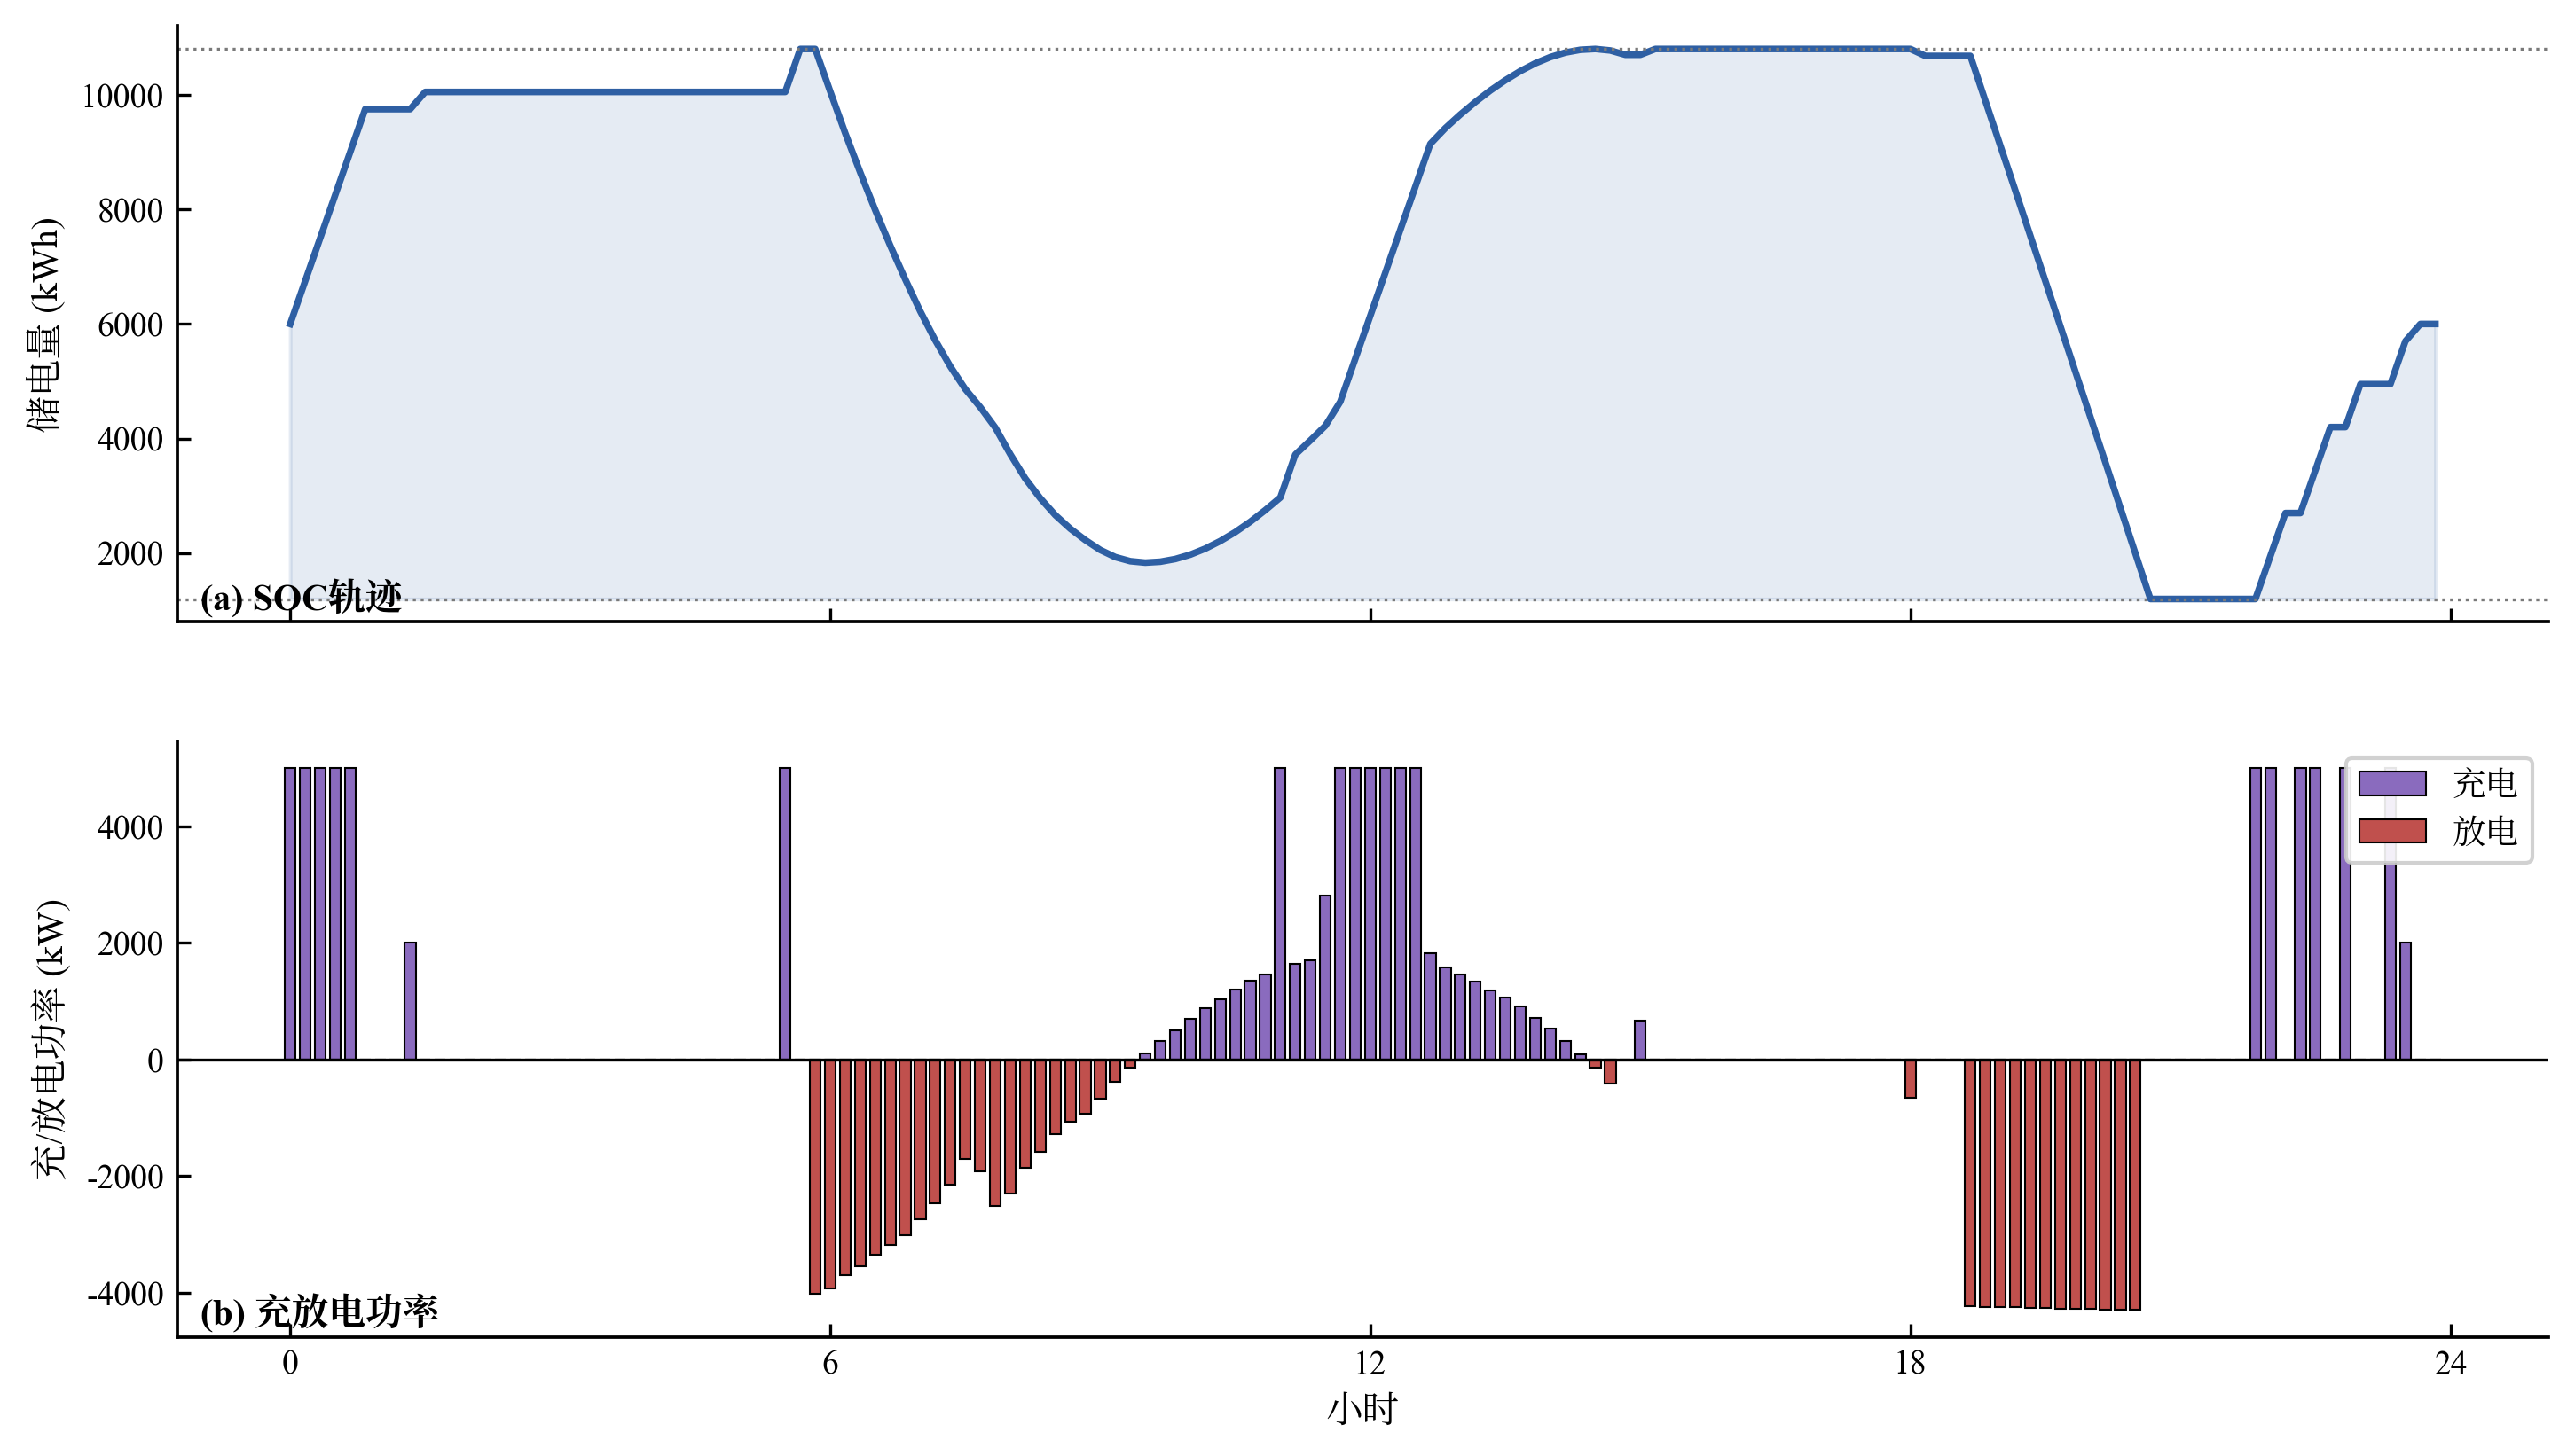
\includegraphics[width=0.62\textwidth]{../求解/问题一/图片/图1-4_储能SOC与充放电功率.png}
    \caption{储能荷电状态轨迹与充放电功率}
    \label{fig:结果1-4}
\end{figure}

微网一天内的能量平衡关系如图\ref{fig:结果1-5}所示，购电、光伏与储能放电三类供给叠加后恰好覆盖小区负载与储能充电需求，任意时刻能量收支闭合，验证了功率平衡约束的严格满足。

\begin{figure}[H]
    \centering
    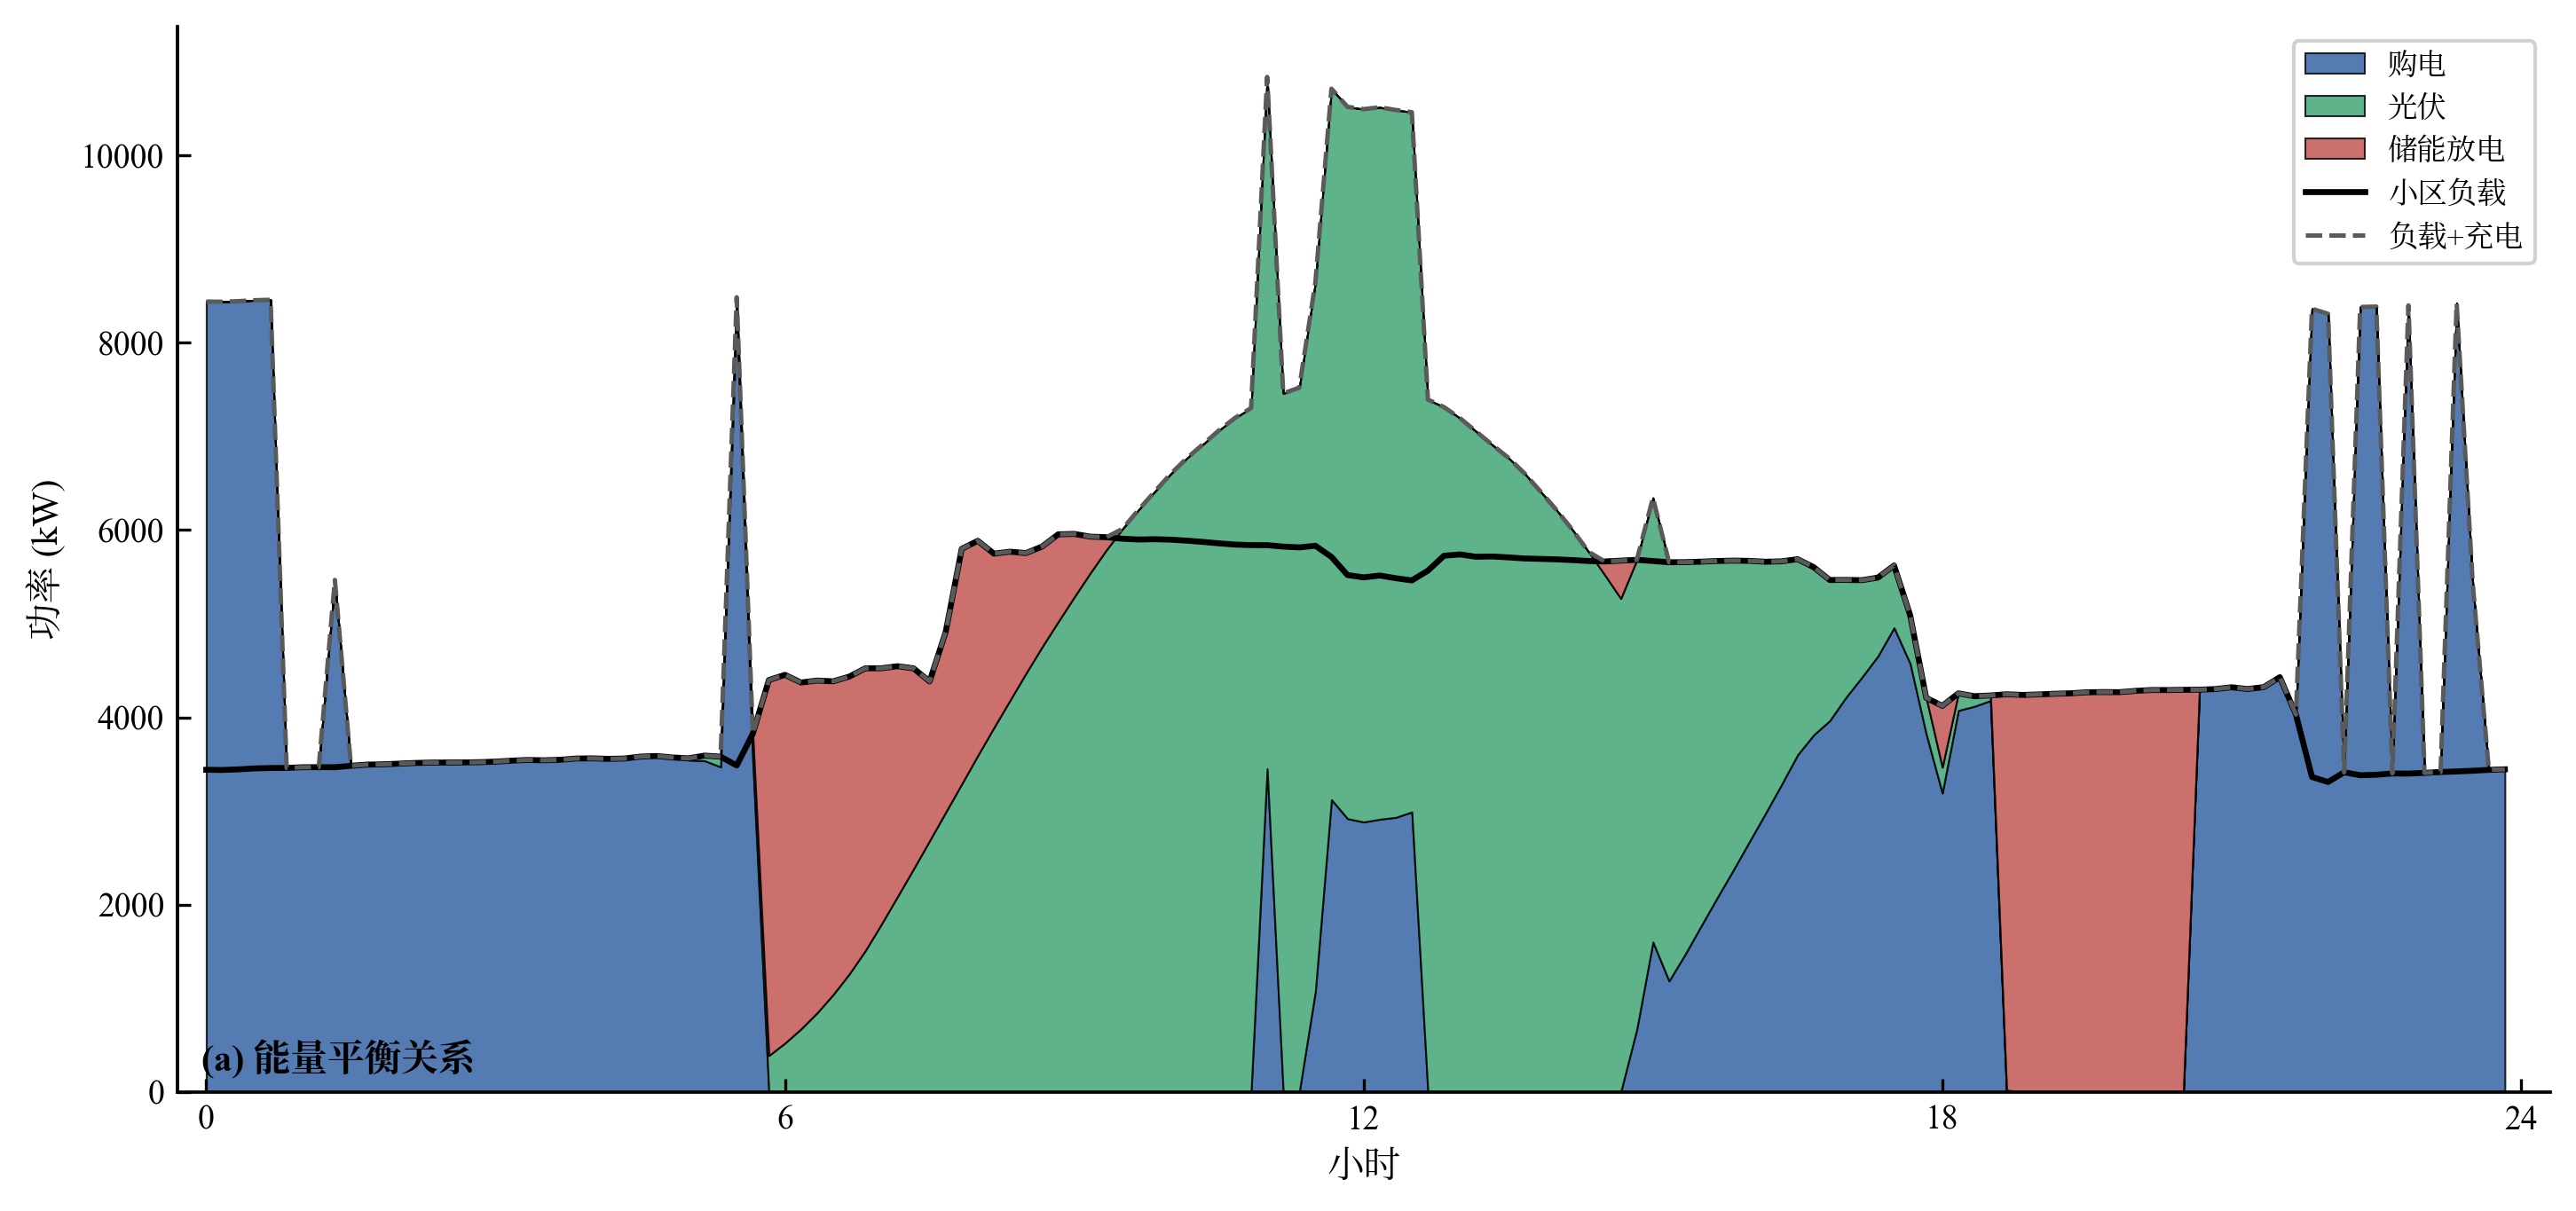
\includegraphics[width=0.70\textwidth]{../求解/问题一/图片/图1-5_能量平衡.png}
    \caption{微网全天能量平衡关系}
    \label{fig:结果1-5}
\end{figure}

储能 0:00 储电量 $E_0$ 由附录1给定为 6000 kWh，属于问题给定的固定条件而非可优化变量。为进一步检验模型对该初值的稳健性，将 $E_0$ 在 $[1200,10800]$ kWh 区间内逐档变动（并保持日循环 $E_{144}=E_0$）重新求解全天购电费，结果如图\ref{fig:结果1-6}所示。可见购电费随 $E_0$ 变化总体平稳，在附录1给定的 6000 kWh 处购电费为 35126.95 元，与最低购电费相比差异很小，说明模型结果对储能初值的选取不敏感，也表明按给定初值求解是合理可靠的。

\begin{figure}[H]
    \centering
    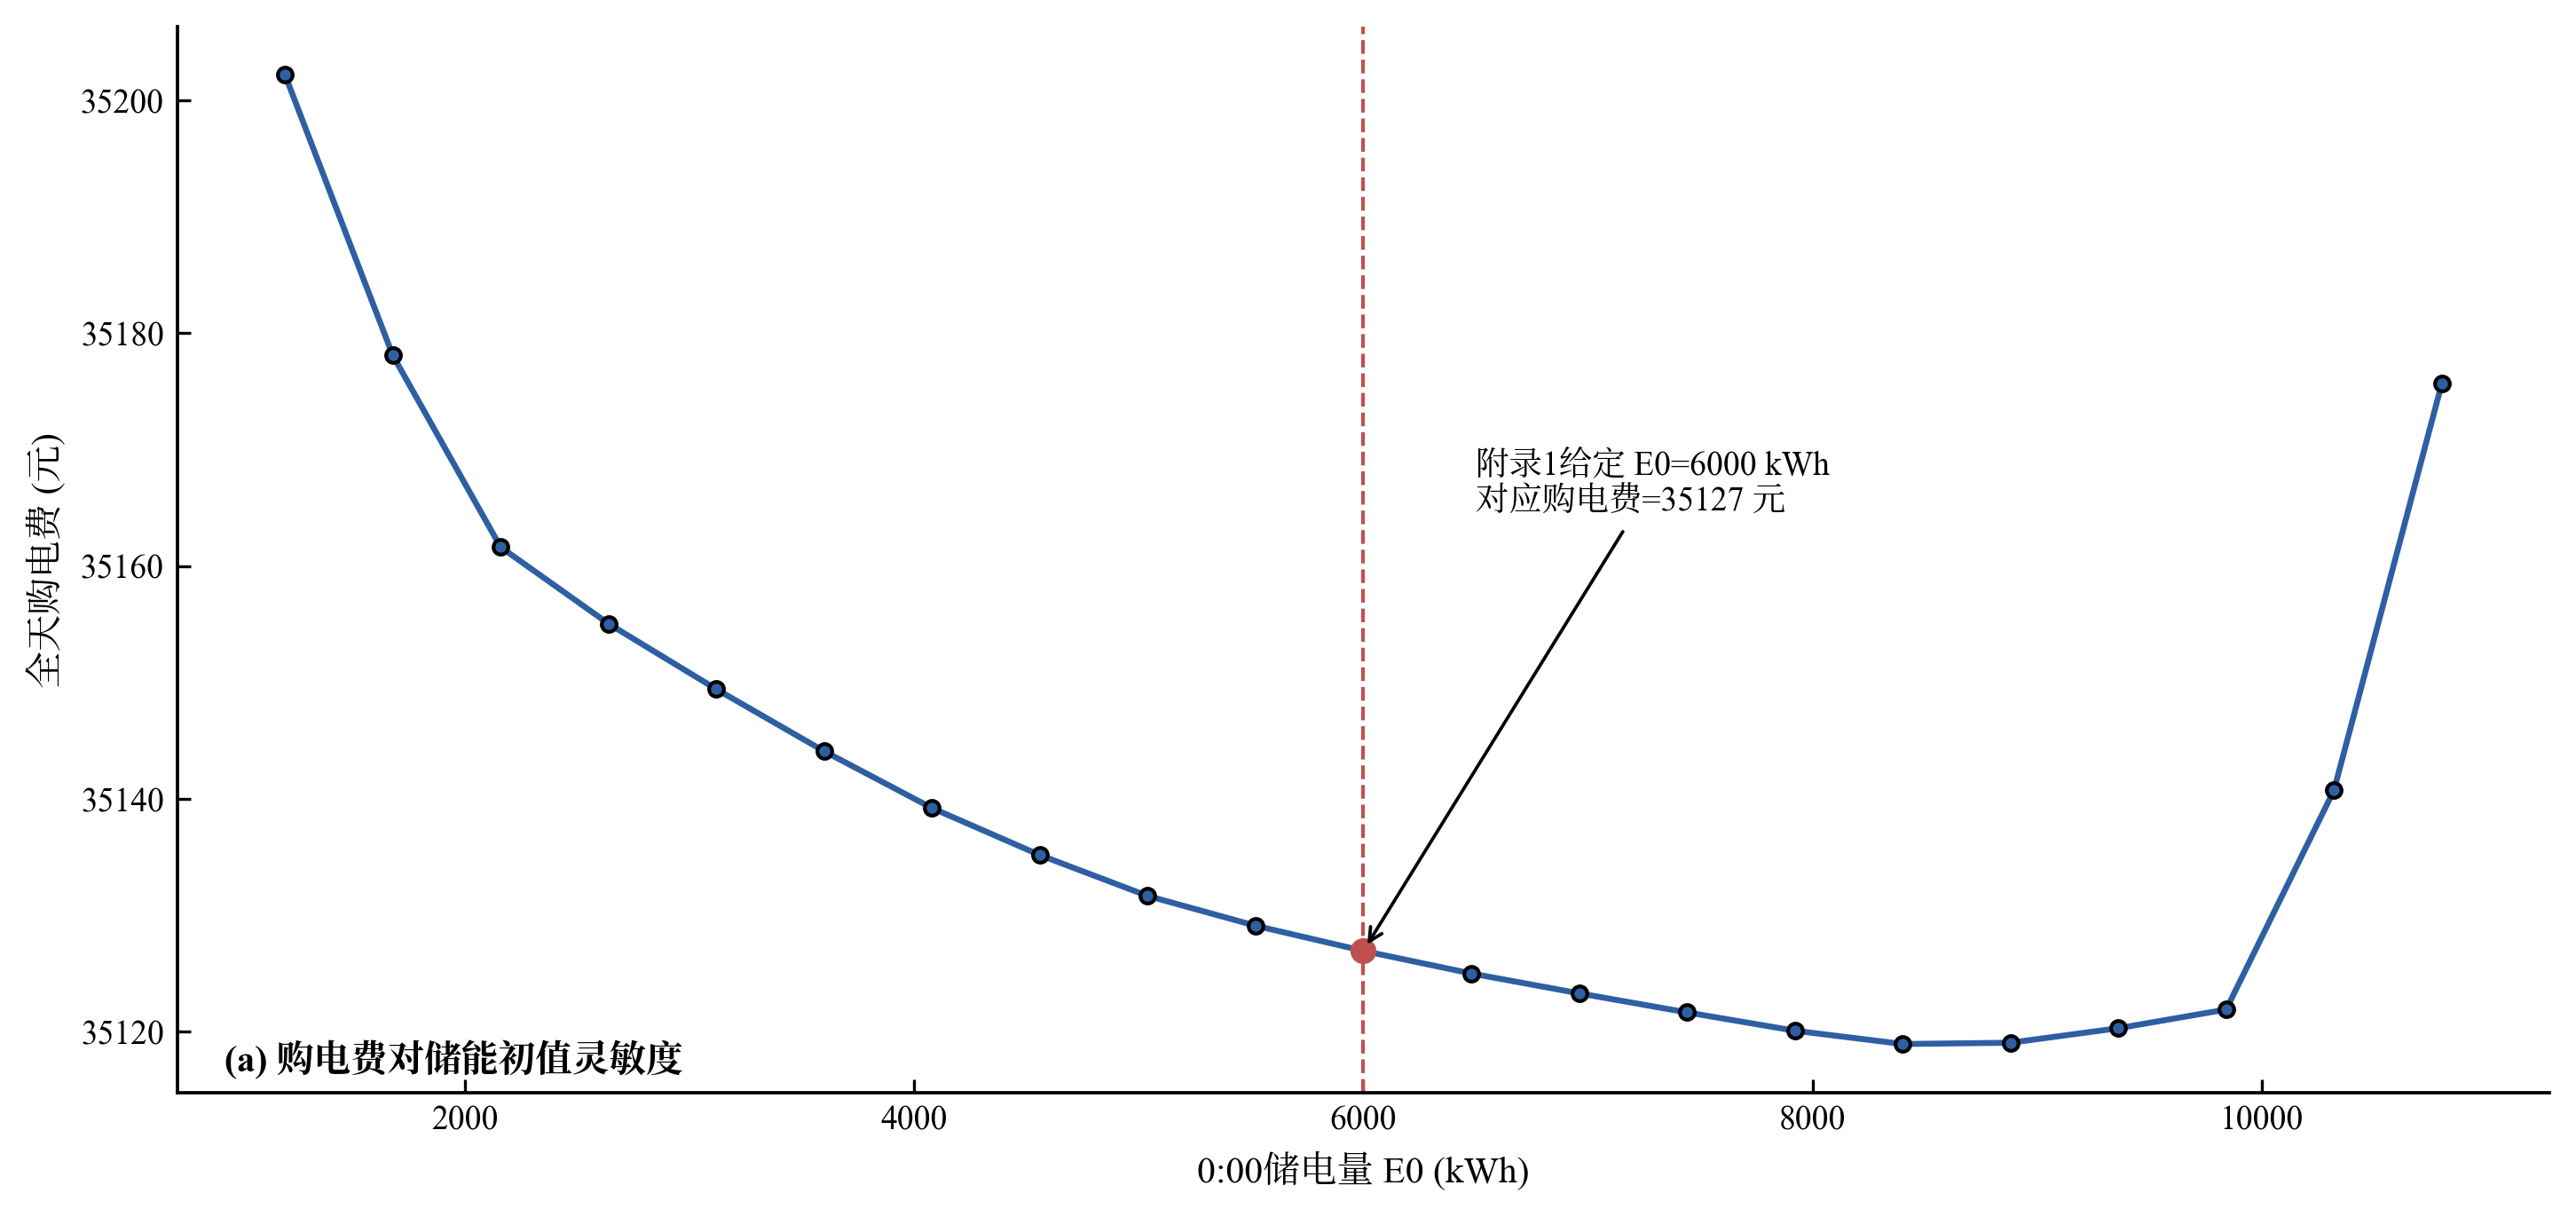
\includegraphics[width=0.70\textwidth]{../求解/问题一/图片/图1-6_购电费灵敏度.png}
    \caption{全天购电费对储能初值的灵敏度}
    \label{fig:结果1-6}
\end{figure}

\begin{longtable}{>{\centering\arraybackslash}p{0.15\textwidth}>{\centering\arraybackslash}p{0.13\textwidth}>{\centering\arraybackslash}p{0.15\textwidth}>{\centering\arraybackslash}p{0.13\textwidth}>{\centering\arraybackslash}p{0.15\textwidth}>{\centering\arraybackslash}p{0.13\textwidth}}
  \caption{微网在指定时间段的购电量及全天的购电量和购电费}
  \label{tab:结果1-1} \\
  \toprule
  时间段 & 购电量 & 时间段 & 购电量 & 时间段 & 购电量 \\
  \midrule
  \endfirsthead
  \caption{微网在指定时间段的购电量及全天的购电量和购电费（续）} \\
  \toprule
  时间段 & 购电量 & 时间段 & 购电量 & 时间段 & 购电量 \\
  \midrule
  \endhead
  \bottomrule
  \endfoot
  10:00--10:10 & 0.00 & 12:00--12:10 & 480.41 & 14:00--14:10 & 0.00 \\
  16:00--16:10 & 445.43 & 18:00--18:10 & 531.89 & 20:00--20:10 & 0.00 \\
  全天购电量 & 59482.70 & 全天购电费 & 35126.95 &  &  \\
\end{longtable}

\begin{longtable}{>{\centering\arraybackslash}p{0.15\textwidth}>{\centering\arraybackslash}p{0.13\textwidth}>{\centering\arraybackslash}p{0.13\textwidth}>{\centering\arraybackslash}p{0.15\textwidth}>{\centering\arraybackslash}p{0.13\textwidth}>{\centering\arraybackslash}p{0.13\textwidth}}
  \caption{储能设备在指定时间段的充放电量及0:00和24:00的储电量}
  \label{tab:结果1-2} \\
  \toprule
  时间段 & 充电量 & 放电量 & 时间段 & 充电量 & 放电量 \\
  \midrule
  \endfirsthead
  \caption{储能设备在指定时间段的充放电量及0:00和24:00的储电量（续）} \\
  \toprule
  时间段 & 充电量 & 放电量 & 时间段 & 充电量 & 放电量 \\
  \midrule
  \endhead
  \bottomrule
  \endfoot
  0:00--4:00 & 4500.00 & 0.00 & 4:00--8:00 & 833.33 & 6365.84 \\
  8:00--12:00 & 4787.96 & 1703.00 & 12:00--16:00 & 5286.04 & 91.10 \\
  16:00--20:00 & 0.00 & 5780.13 & 20:00--24:00 & 5333.33 & 2859.87 \\
  0:00储电量 & 6000.00 &  & 24:00储电量 & 6000.00 &  \\
\end{longtable}

由表\ref{tab:结果1-1}可知，微网全天计划购电量为 59482.70 kWh，全天购电费为 35126.95 元；在 10:00--10:10、14:00--14:10 与 20:00--20:10 等光伏充足或储能放电充足的时段购电量为零，而在 12:00--12:10、16:00--16:10、18:00--18:10 等负荷高企时段需要少量购电。由表\ref{tab:结果1-2}可知，储能设备在 0:00 与 24:00 的储电量均为 6000.00 kWh，与附录1给定的 0:00 储电量一致，同时满足日循环约束；储能主要在 0:00--4:00、8:00--12:00 与 20:00--24:00 等低电价时段充电，在 4:00--8:00、16:00--20:00 等高电价时段放电，体现了低充高放的套利规律。

综合以上结果，问题一的线性规划模型在满足负载供电与储能运行约束的前提下，给出了全天购电费用最小的购电与充放电策略，储能设备在低价充电、高价放电的套利过程中使购电费用显著降低，模型与结果均合理可靠。



% ┈┈┈┈┈┈┈┈┈┈┈┈┈┈┈┈┈┈┈┈┈┈┈┈┈┈┈┈┈┈┈┈┈┈┈
% 【本章节写作提示词】
% ════════════════════════════════════════════
% 【作用】这是每个小问的包装（二级标题）：题目有几个小问，就在 模型的建立与求解 组成里放几个 5.X 子块，
%   并为每个小问复制本块为 5.X.问题X的建立求解（X = 第几小问）。
% 【结构】固定 \subsection{问题X的模型的建立和求解}，内部由下方「__SUBS__ 占位」注入四个三级子块，顺序固定为：
%   ① 具体分析 → ② 模型准备 → ③ 模型建立 → ④ 模型求解（见各子块顶部注释，组合题型按题目主要类型选择）。
% 【来源】图片 ../求解/问题X/图片/xxx.png；数据 ../求解/问题X/结果/ 的 CSV。
% ════════════════════════════════════════════
